% Ly thuyet de chuan bi cho viec xay dung phan cung 
% Slide 1: Kiến trúc Hệ thống
\begin{frame}{Kiến trúc Hệ thống Phát hiện Té ngã}
\begin{columns}[T]
\column{0.5\textwidth}
\begin{block}{Phân loại}
\begin{itemize}
    \item Camera-based
    \item Wearable-based
\end{itemize}
\end{block}
\column{0.5\textwidth}
\begin{block}{Thành phần chính}
\begin{enumerate}
    \item Thiết bị thu thập (IMU/Camera)
    \item Máy chủ xử lý (Deep Learning)
    \item Truyền thông (Wi-Fi, 4G)
\end{enumerate}
\end{block}
\end{columns}
\end{frame}

% Slide 2: Edge Processing
\begin{frame}{Xử lý Cục bộ (Edge)}
\begin{itemize}
    \item \textbf{ESP32}: lõi kép, FreeRTOS, xử lý song song.
    \item \textbf{IMU}: 
    \begin{itemize}
        \item Gia tốc kế, Con quay, Từ kế
        \item Sensor Fusion (Kalman/Madgwick)
    \end{itemize}
    \item \textbf{Ngưỡng phát hiện té ngã}:
    \[
    \|\mathbf{a}\| > a_{\text{shock}}, \quad \|\mathbf{a}\| \approx 1g
    \]
    \item \textbf{GPS}: định vị NMEA, hỗ trợ cứu hộ.
\end{itemize}
\end{frame}

% Slide 3: Host/Cloud Processing
\begin{frame}{Xử lý Máy chủ (Host/Cloud)}
\begin{columns}[T]
\column{0.5\textwidth}
\begin{block}{Camera Input}
ESP32-S3 + OV5640 (5MP) \\
→ stream JPEG qua Wi-Fi
\end{block}
\column{0.5\textwidth}
\begin{block}{Máy chủ}
\begin{itemize}
    \item GPU (Jetson Nano, Cloud)
    \item TensorFlow/PyTorch + OpenCV
    \item Đồng bộ IMU (MQTT/JSON) + Camera (JPEG)
\end{itemize}
\end{block}
\end{columns}
\end{frame}

% Slide 4: Truyền thông & Dự phòng
\begin{frame}{Hệ thống Truyền thông \& Dự phòng}
\begin{block}{Kênh truyền}
\begin{itemize}
    \item Wi-Fi: kênh chính
    \item 4G/LTE (EC800K): dự phòng, SMS/cuộc gọi khẩn
\end{itemize}
\end{block}

\begin{alertblock}{Logic vận hành}
\begin{enumerate}
    \item ESP32 phát hiện sơ cấp
    \item Truyền dữ liệu: Wi-Fi $\to$ 4G
    \item Server xác minh (IMU + HPE)
    \item Kích hoạt cảnh báo
\end{enumerate}
\end{alertblock}
\end{frame}

% Slide 5: Môi trường Phát triển
\begin{frame}{Môi trường Phát triển Phần mềm}
\begin{block}{ESP-IDF Framework}
\begin{itemize}
    \item Hỗ trợ FreeRTOS (đa nhiệm, lõi kép)
    \item Low-level Access (I2C/SPI, MQTT/HTTP tối ưu)
    \item Chuyên nghiệp hơn Arduino IDE
\end{itemize}
\end{block}
\end{frame}

% Section 1
\section{Tổng quan Kiến trúc Hệ thống}

\begin{frame}{Tổng quan Kiến trúc Hệ thống Phát hiện Té ngã}
\begin{block}{Phân loại hệ thống}
Hệ thống phát hiện té ngã hiện đại được chia thành hai nhóm chính:
\begin{itemize}
\item \textbf{Hệ thống dựa trên Camera}
\item \textbf{Hệ thống dựa trên Thiết bị đeo}
\end{itemize}
\end{block}

\begin{block}{Ba thành phần cốt lõi}
\begin{enumerate}
\item \textbf{Thiết bị Thu thập Dữ liệu}: Thu thập dữ liệu chuyển động (IMU) và/hoặc hình ảnh (Camera)
\item \textbf{Máy chủ Xử lý}: Thực hiện các thuật toán học sâu và logic ra quyết định phức tạp
\item \textbf{Hệ thống Truyền thông}: Đảm bảo luồng dữ liệu hai chiều và kích hoạt cảnh báo
\end{enumerate}
\end{block}
\end{frame}

% Section 2
\section{Vi điều khiển và Cảm biến}

\begin{frame}{Vi điều khiển ESP32}
\begin{columns}
\column{0.6\textwidth}
\begin{block}{Tại sao chọn ESP32?}
\begin{itemize}
\item Kiến trúc \textbf{lõi kép Xtensa LX6}
\item Xử lý song song hiệu quả
\item Tích hợp Wi-Fi, Bluetooth
\item Hỗ trợ giao thức MQTT, HTTP
\end{itemize}
\end{block}

\begin{block}{Phân công nhiệm vụ}
\begin{itemize}
\item \textbf{Lõi 1}: Xử lý thời gian thực (IMU, Kalman Filter)
\item \textbf{Lõi 2}: Truyền thông không dây
\end{itemize}
\end{block}

\column{0.4\textwidth}
\begin{center}
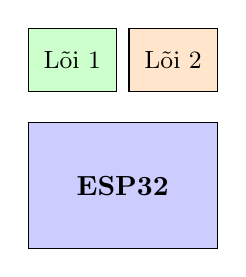
\begin{tikzpicture}[scale=0.8]
\draw[fill=blue!20] (0,0) rectangle (3,2);
\node at (1.5,1) {\textbf{ESP32}};
\draw[fill=green!20] (0,2.5) rectangle (1.4,3.5);
\node at (0.7,3) {\small Lõi 1};
\draw[fill=orange!20] (1.6,2.5) rectangle (3,3.5);
\node at (2.3,3) {\small Lõi 2};
\end{tikzpicture}
\end{center}
\end{columns}
\end{frame}

\begin{frame}{Cảm biến IMU}
\begin{block}{IMU (Inertial Measurement Unit)}
Tích hợp ba loại cảm biến quan trọng:
\end{block}

\begin{columns}
\column{0.33\textwidth}
\begin{alertblock}{Gia tốc kế}
\begin{itemize}
\item Đo gia tốc tuyến tính
\item Hiệu chuẩn từ số nguyên sang đơn vị $g$
\item Vector 3D: $\mathbf{a} = [a_x, a_y, a_z]$
\end{itemize}
\end{alertblock}

\column{0.33\textwidth}
\begin{alertblock}{Con quay hồi chuyển}
\begin{itemize}
\item Đo tốc độ góc
\item Dựa trên hiệu ứng Coriolis
\item Vector 3D: $\boldsymbol{\omega} = [\omega_x, \omega_y, \omega_z]$
\end{itemize}
\end{alertblock}

\column{0.33\textwidth}
\begin{alertblock}{Từ kế}
\begin{itemize}
\item Tham chiếu hướng từ trường
\item Hiệu chỉnh sai số trôi
\item Sensor Fusion (Madgwick, Kalman)
\end{itemize}
\end{alertblock}
\end{columns}
\end{frame}

\begin{frame}{Thuật toán Phát hiện Té ngã}
\begin{block}{Phát hiện dựa trên ngưỡng IMU}
Phân tích sự thay đổi đột ngột của gia tốc và tốc độ góc
\end{block}

\begin{columns}
\column{0.5\textwidth}
\begin{alertblock}{Shock Event}
Gia tốc tổng vượt ngưỡng cao:
$$\|\mathbf{a}\| > a_{\text{shock}}$$

Với: $$\|\mathbf{a}\| = \sqrt{a_x^2 + a_y^2 + a_z^2}$$
\end{alertblock}

\column{0.5\textwidth}
\begin{alertblock}{Post-fall State}
\begin{itemize}
\item Gia tốc tổng giảm về gần 1g
\item Biểu thị trạng thái nằm ngang
\item Tốc độ góc có thay đổi lớn
\end{itemize}
\end{alertblock}
\end{columns}

\vspace{0.5cm}
\begin{exampleblock}{Cảm biến GPS}
Module GPS (u-blox NEO-6M) sử dụng \textbf{đo tam giác} từ ít nhất 4 vệ tinh, cung cấp tọa độ cho dịch vụ cứu hộ khẩn cấp.
\end{exampleblock}
\end{frame}

% Section 3
\section{Hệ thống Camera và Xử lý}

\begin{frame}{Hệ thống Camera và Máy chủ}
\begin{columns}
\column{0.5\textwidth}
\begin{block}{Camera Input}
\begin{itemize}
\item ESP32-S3 + OV5640 5MP
\item Nén JPEG
\item Truyền qua Wi-Fi (RTSP/HTTP)
\item Xác minh hình ảnh
\end{itemize}
\end{block}

\begin{block}{Luồng dữ liệu}
\begin{itemize}
\item Luồng JSON/MQTT (IMU)
\item Luồng JPEG (Camera)
\item Đồng bộ hóa dữ liệu
\item Giảm báo động giả
\end{itemize}
\end{block}

\column{0.5\textwidth}
\begin{block}{Kiến trúc Máy chủ}
\textbf{Phần cứng:}
\begin{itemize}
\item AWS, Google Cloud
\item NVIDIA Jetson Nano
\item GPU cho tính toán Tensor
\end{itemize}

\textbf{Phần mềm:}
\begin{itemize}
\item TensorFlow/PyTorch
\item OpenCV
\item Thuật toán HPE
\item Học sâu
\end{itemize}
\end{block}
\end{columns}
\end{frame}

% Section 4
\section{Hệ thống Truyền thông}

\begin{frame}{Module Truyền thông}
\begin{columns}
\column{0.5\textwidth}
\begin{alertblock}{Wi-Fi (ESP32) - Kênh chính}
\begin{itemize}
\item Truyền tải dữ liệu dung lượng lớn
\item Video/hình ảnh
\item Giao tiếp MQTT với máy chủ
\item Độ trễ thấp
\end{itemize}
\end{alertblock}

\column{0.5\textwidth}
\begin{alertblock}{4G/LTE (EC800K) - Dự phòng}
\begin{itemize}
\item Hoạt động khi Wi-Fi không khả dụng
\item Hỗ trợ định vị GPS
\item Cuộc gọi khẩn cấp tự động
\item SMS cảnh báo qua AT commands
\end{itemize}
\end{alertblock}
\end{columns}
\end{frame}

\begin{frame}{Logic Hoạt động}
\begin{enumerate}
\item \textbf{Thu thập/Xử lý Sơ cấp}
\begin{itemize}
\item ESP32 thu thập dữ liệu IMU/Camera
\item Phát hiện té ngã dựa trên ngưỡng IMU
\end{itemize}

\item \textbf{Quyết định Truyền thông}
\begin{itemize}
\item Nếu phát hiện té ngã → truyền dữ liệu lên máy chủ
\item Ưu tiên Wi-Fi, dự phòng 4G
\end{itemize}

\item \textbf{Xác minh Máy chủ}
\begin{itemize}
\item Phân tích hình ảnh (HPE)
\item Kết hợp dữ liệu IMU
\item Multi-stage Fall Detection Logic
\end{itemize}

\item \textbf{Kích hoạt Cảnh báo}
\begin{itemize}
\item Xác nhận té ngã → ra lệnh cho ESP32
\item Kích hoạt Module EC800K gửi SMS/Cuộc gọi
\end{itemize}
\end{enumerate}
\end{frame}

% Section 5
\section{Môi trường Phát triển}

\begin{frame}{ESP-IDF Framework}
\begin{block}{Tại sao chọn ESP-IDF thay vì Arduino IDE?}
\end{block}

\begin{columns}
\column{0.5\textwidth}
\begin{alertblock}{Hỗ trợ RTOS}
\begin{itemize}
\item Tích hợp FreeRTOS
\item Tận dụng kiến trúc lõi kép
\item Đa nhiệm thực sự
\item Tác vụ IMU song song với Wi-Fi
\end{itemize}
\end{alertblock}

\column{0.5\textwidth}
\begin{alertblock}{Truy cập Cấp thấp}
\begin{itemize}
\item Truy cập trực tiếp thanh ghi phần cứng
\item Cấu hình chi tiết cảm biến (I2C/SPI)
\item Tối ưu hóa giao thức mạng
\item Hiệu suất thời gian thực
\end{itemize}
\end{alertblock}
\end{columns}
\end{frame}
